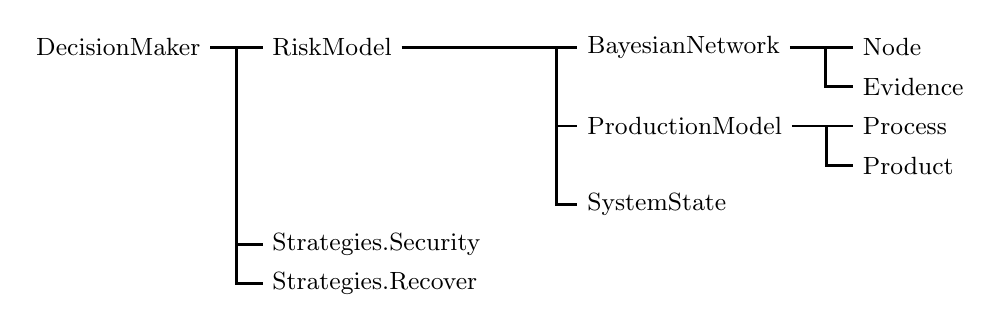
\begin{tikzpicture}[line width = 1pt]

\small

\node[anchor = west] (DM) at ( 0, 9.0) {\code{DecisionMaker}};
\node[anchor = west] (RM) at ( 3, 9.0) {\code{RiskModel}};
\node[anchor = west] (SS) at ( 3, 6.5) {\code{Strategies.Security}};
\node[anchor = west] (SR) at ( 3, 6.0) {\code{Strategies.Recover}};
\node[anchor = west] (BN) at ( 7, 9.0) {\code{BayesianNetwork}};
\node[anchor = west] (PM) at ( 7, 8.0) {\code{ProductionModel}};
\node[anchor = west] (ST) at ( 7, 7.0) {\code{SystemState}};

\node[anchor = west] (ND) at (10.5, 9.0) {\code{Node}};
\node[anchor = west] (EV) at (10.5, 8.5) {\code{Evidence}};
\node[anchor = west] (PR) at (10.5, 8.0) {\code{Process}};
\node[anchor = west] (PD) at (10.5, 7.5) {\code{Product}};

\draw (DM) -- (RM)
      (DM) -- ++(0:1.5cm) |- (SS)
      (DM) -- ++(0:1.5cm) |- (SR);

\draw (RM) -- (BN)
      (RM) -- ++(0:2.85cm) |- (PM)
      (RM) -- ++(0:2.85cm) |- (ST);   
      
\draw (BN) -- (ND)
      (BN) -- ++(0:1.8cm) |- (EV);
      
\draw (PM) -- (PR)
      (PM) -- ++(0:1.8cm) |- (PD);      

\end{tikzpicture} 